% Source for images/1D-4D.{pdf,png} — geometrical objects in 1 to 4 dimensions,
% shown in 01-Prelude.qmd (chunk `fig-1D-4D`).
%
% This is an author redraw (2026-07-10) of the former low-res raster, which was
% an unattributed web graphic (~98 effective dpi in print; see
% issues/CMYK-checklist.md and issues/fig-permission-list.md). Every coordinate
% is in the original raster's pixel units (482x305 canvas, y down), extracted
% programmatically from the image, so geometry and layout replicate it exactly.
% The tesseract uses hidden-line style, as in the original: the outer and inner
% back faces show only their top and left edges, with no corner edge or
% connector at the hidden back-bottom-right vertex.
%
% Not built by make-diagrams.sh (that script handles the part-page and
% chapter-opener mindmaps only). Rebuild both outputs from this directory:
%
%   # vector PDF, CMYK colors — used in the print/PDF book
%   xelatex -jobname 1D-4D "\def\cmykcolors{}% Source for images/1D-4D.{pdf,png} — geometrical objects in 1 to 4 dimensions,
% shown in 01-Prelude.qmd (chunk `fig-1D-4D`).
%
% This is an author redraw (2026-07-10) of the former low-res raster, which was
% an unattributed web graphic (~98 effective dpi in print; see
% issues/CMYK-checklist.md and issues/fig-permission-list.md). Every coordinate
% is in the original raster's pixel units (482x305 canvas, y down), extracted
% programmatically from the image, so geometry and layout replicate it exactly.
% The tesseract uses hidden-line style, as in the original: the outer and inner
% back faces show only their top and left edges, with no corner edge or
% connector at the hidden back-bottom-right vertex.
%
% Not built by make-diagrams.sh (that script handles the part-page and
% chapter-opener mindmaps only). Rebuild both outputs from this directory:
%
%   # vector PDF, CMYK colors — used in the print/PDF book
%   xelatex -jobname 1D-4D "\def\cmykcolors{}% Source for images/1D-4D.{pdf,png} — geometrical objects in 1 to 4 dimensions,
% shown in 01-Prelude.qmd (chunk `fig-1D-4D`).
%
% This is an author redraw (2026-07-10) of the former low-res raster, which was
% an unattributed web graphic (~98 effective dpi in print; see
% issues/CMYK-checklist.md and issues/fig-permission-list.md). Every coordinate
% is in the original raster's pixel units (482x305 canvas, y down), extracted
% programmatically from the image, so geometry and layout replicate it exactly.
% The tesseract uses hidden-line style, as in the original: the outer and inner
% back faces show only their top and left edges, with no corner edge or
% connector at the hidden back-bottom-right vertex.
%
% Not built by make-diagrams.sh (that script handles the part-page and
% chapter-opener mindmaps only). Rebuild both outputs from this directory:
%
%   # vector PDF, CMYK colors — used in the print/PDF book
%   xelatex -jobname 1D-4D "\def\cmykcolors{}% Source for images/1D-4D.{pdf,png} — geometrical objects in 1 to 4 dimensions,
% shown in 01-Prelude.qmd (chunk `fig-1D-4D`).
%
% This is an author redraw (2026-07-10) of the former low-res raster, which was
% an unattributed web graphic (~98 effective dpi in print; see
% issues/CMYK-checklist.md and issues/fig-permission-list.md). Every coordinate
% is in the original raster's pixel units (482x305 canvas, y down), extracted
% programmatically from the image, so geometry and layout replicate it exactly.
% The tesseract uses hidden-line style, as in the original: the outer and inner
% back faces show only their top and left edges, with no corner edge or
% connector at the hidden back-bottom-right vertex.
%
% Not built by make-diagrams.sh (that script handles the part-page and
% chapter-opener mindmaps only). Rebuild both outputs from this directory:
%
%   # vector PDF, CMYK colors — used in the print/PDF book
%   xelatex -jobname 1D-4D "\def\cmykcolors{}\input{fig-1D-4D.tex}"
%   mv 1D-4D.pdf ../../images/
%
%   # high-res sRGB PNG (600 dpi) — used in the HTML book
%   xelatex -jobname 1D-4D-rgb "\input{fig-1D-4D.tex}"
%   magick -density 600 1D-4D-rgb.pdf -background white -flatten ../../images/1D-4D.png
%   rm -f 1D-4D-rgb.pdf *.aux *.log
%
% The drawing is pure black, so the CMYK variant prints as 100% K ink.
\ifdefined\cmykcolors
  \PassOptionsToPackage{cmyk}{xcolor}
\else
  \PassOptionsToPackage{rgb}{xcolor}
\fi
\documentclass[border=0pt]{standalone}
\usepackage{fontspec}
\setsansfont{Arial}  % labels match the original raster's Arial; needs xelatex
\usepackage{tikz}

\begin{document}
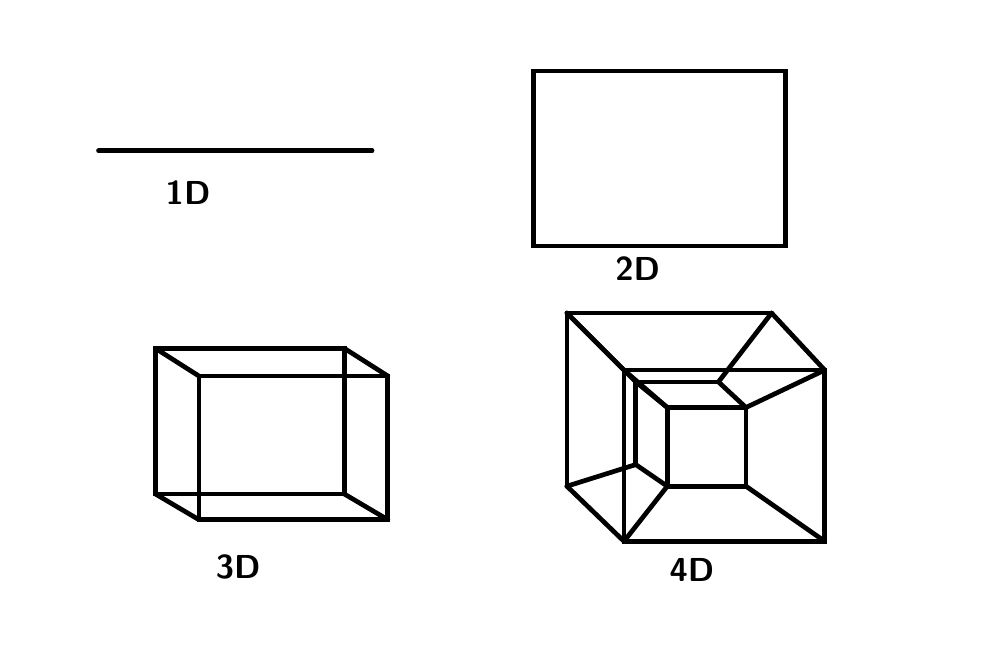
\begin{tikzpicture}[x=0.025cm, y=-0.025cm, line width=1.7pt, line cap=round,
                    lbl/.style={font=\fontsize{12}{12}\selectfont\sffamily\bfseries, inner sep=0pt}]

% full original canvas, including its (asymmetric) margins
\useasboundingbox (0,0) rectangle (482,305);

% ---- 1D: line ----
\draw (36,62.5) -- (175,62.5);
\node[lbl] at (81.5,84) {1D};

% ---- 2D: rectangle ----
\draw (257,22) rectangle (385,111);
\node[lbl] at (310,122.5) {2D};

% ---- 3D: cube (full wireframe, back face up-left) ----
\draw (65,163) rectangle (161,237);   % back face
\draw (87,177) rectangle (183,250);   % front face
\draw (65,163) -- (87,177)  (161,163) -- (183,177)
      (65,237) -- (87,250)  (161,237) -- (183,250);
\node[lbl] at (107,274) {3D};

% ---- 4D: tesseract (outer + inner cube, hidden lines removed) ----
% outer cube: front face A1..A4, back face B1(TL) B2(TR) B4(BL); B3 hidden
\coordinate (A1) at (303,174); \coordinate (A2) at (405,174);
\coordinate (A3) at (405,261); \coordinate (A4) at (303,261);
\coordinate (B1) at (274,145); \coordinate (B2) at (378,145);
\coordinate (B4) at (274,233);
% inner cube: front face a1..a4, back face b1(TL) b2(TR) b4(BL); b3 hidden
\coordinate (a1) at (325,193); \coordinate (a2) at (365,193);
\coordinate (a3) at (365,233); \coordinate (a4) at (325,233);
\coordinate (b1) at (309,180); \coordinate (b2) at (351,180);
\coordinate (b4) at (309,222);

\draw (A1) rectangle (A3);            % outer front face
\draw (B2) -- (B1) -- (B4);           % outer back face: top + left edges only
\draw (B1) -- (A1) (B2) -- (A2) (B4) -- (A4);   % outer corner edges
\draw (a1) rectangle (a3);            % inner front face
\draw (b2) -- (b1) -- (b4);           % inner back face: top + left edges only
\draw (b1) -- (a1) (b2) -- (a2) (b4) -- (a4);   % inner corner edges
% tesseract connectors, outer vertex -> inner vertex
\draw (B1) -- (b1) (B2) -- (b2) (B4) -- (b4)
      (A1) -- (a1) (A2) -- (a2) (A3) -- (a3) (A4) -- (a4);
\node[lbl] at (337.5,275.5) {4D};

\end{tikzpicture}
\end{document}
"
%   mv 1D-4D.pdf ../../images/
%
%   # high-res sRGB PNG (600 dpi) — used in the HTML book
%   xelatex -jobname 1D-4D-rgb "% Source for images/1D-4D.{pdf,png} — geometrical objects in 1 to 4 dimensions,
% shown in 01-Prelude.qmd (chunk `fig-1D-4D`).
%
% This is an author redraw (2026-07-10) of the former low-res raster, which was
% an unattributed web graphic (~98 effective dpi in print; see
% issues/CMYK-checklist.md and issues/fig-permission-list.md). Every coordinate
% is in the original raster's pixel units (482x305 canvas, y down), extracted
% programmatically from the image, so geometry and layout replicate it exactly.
% The tesseract uses hidden-line style, as in the original: the outer and inner
% back faces show only their top and left edges, with no corner edge or
% connector at the hidden back-bottom-right vertex.
%
% Not built by make-diagrams.sh (that script handles the part-page and
% chapter-opener mindmaps only). Rebuild both outputs from this directory:
%
%   # vector PDF, CMYK colors — used in the print/PDF book
%   xelatex -jobname 1D-4D "\def\cmykcolors{}\input{fig-1D-4D.tex}"
%   mv 1D-4D.pdf ../../images/
%
%   # high-res sRGB PNG (600 dpi) — used in the HTML book
%   xelatex -jobname 1D-4D-rgb "\input{fig-1D-4D.tex}"
%   magick -density 600 1D-4D-rgb.pdf -background white -flatten ../../images/1D-4D.png
%   rm -f 1D-4D-rgb.pdf *.aux *.log
%
% The drawing is pure black, so the CMYK variant prints as 100% K ink.
\ifdefined\cmykcolors
  \PassOptionsToPackage{cmyk}{xcolor}
\else
  \PassOptionsToPackage{rgb}{xcolor}
\fi
\documentclass[border=0pt]{standalone}
\usepackage{fontspec}
\setsansfont{Arial}  % labels match the original raster's Arial; needs xelatex
\usepackage{tikz}

\begin{document}
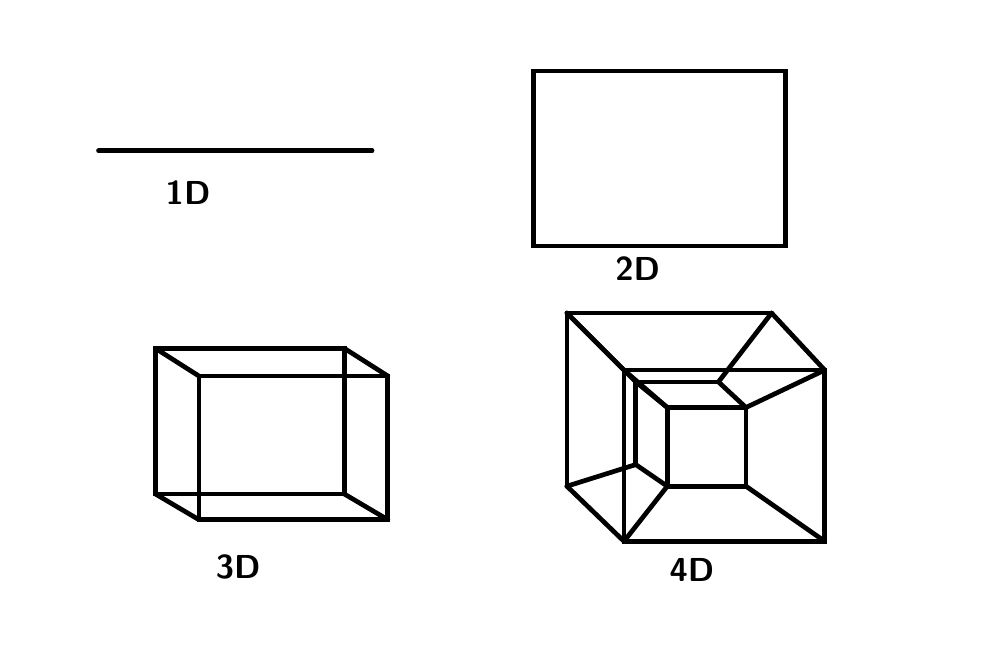
\begin{tikzpicture}[x=0.025cm, y=-0.025cm, line width=1.7pt, line cap=round,
                    lbl/.style={font=\fontsize{12}{12}\selectfont\sffamily\bfseries, inner sep=0pt}]

% full original canvas, including its (asymmetric) margins
\useasboundingbox (0,0) rectangle (482,305);

% ---- 1D: line ----
\draw (36,62.5) -- (175,62.5);
\node[lbl] at (81.5,84) {1D};

% ---- 2D: rectangle ----
\draw (257,22) rectangle (385,111);
\node[lbl] at (310,122.5) {2D};

% ---- 3D: cube (full wireframe, back face up-left) ----
\draw (65,163) rectangle (161,237);   % back face
\draw (87,177) rectangle (183,250);   % front face
\draw (65,163) -- (87,177)  (161,163) -- (183,177)
      (65,237) -- (87,250)  (161,237) -- (183,250);
\node[lbl] at (107,274) {3D};

% ---- 4D: tesseract (outer + inner cube, hidden lines removed) ----
% outer cube: front face A1..A4, back face B1(TL) B2(TR) B4(BL); B3 hidden
\coordinate (A1) at (303,174); \coordinate (A2) at (405,174);
\coordinate (A3) at (405,261); \coordinate (A4) at (303,261);
\coordinate (B1) at (274,145); \coordinate (B2) at (378,145);
\coordinate (B4) at (274,233);
% inner cube: front face a1..a4, back face b1(TL) b2(TR) b4(BL); b3 hidden
\coordinate (a1) at (325,193); \coordinate (a2) at (365,193);
\coordinate (a3) at (365,233); \coordinate (a4) at (325,233);
\coordinate (b1) at (309,180); \coordinate (b2) at (351,180);
\coordinate (b4) at (309,222);

\draw (A1) rectangle (A3);            % outer front face
\draw (B2) -- (B1) -- (B4);           % outer back face: top + left edges only
\draw (B1) -- (A1) (B2) -- (A2) (B4) -- (A4);   % outer corner edges
\draw (a1) rectangle (a3);            % inner front face
\draw (b2) -- (b1) -- (b4);           % inner back face: top + left edges only
\draw (b1) -- (a1) (b2) -- (a2) (b4) -- (a4);   % inner corner edges
% tesseract connectors, outer vertex -> inner vertex
\draw (B1) -- (b1) (B2) -- (b2) (B4) -- (b4)
      (A1) -- (a1) (A2) -- (a2) (A3) -- (a3) (A4) -- (a4);
\node[lbl] at (337.5,275.5) {4D};

\end{tikzpicture}
\end{document}
"
%   magick -density 600 1D-4D-rgb.pdf -background white -flatten ../../images/1D-4D.png
%   rm -f 1D-4D-rgb.pdf *.aux *.log
%
% The drawing is pure black, so the CMYK variant prints as 100% K ink.
\ifdefined\cmykcolors
  \PassOptionsToPackage{cmyk}{xcolor}
\else
  \PassOptionsToPackage{rgb}{xcolor}
\fi
\documentclass[border=0pt]{standalone}
\usepackage{fontspec}
\setsansfont{Arial}  % labels match the original raster's Arial; needs xelatex
\usepackage{tikz}

\begin{document}
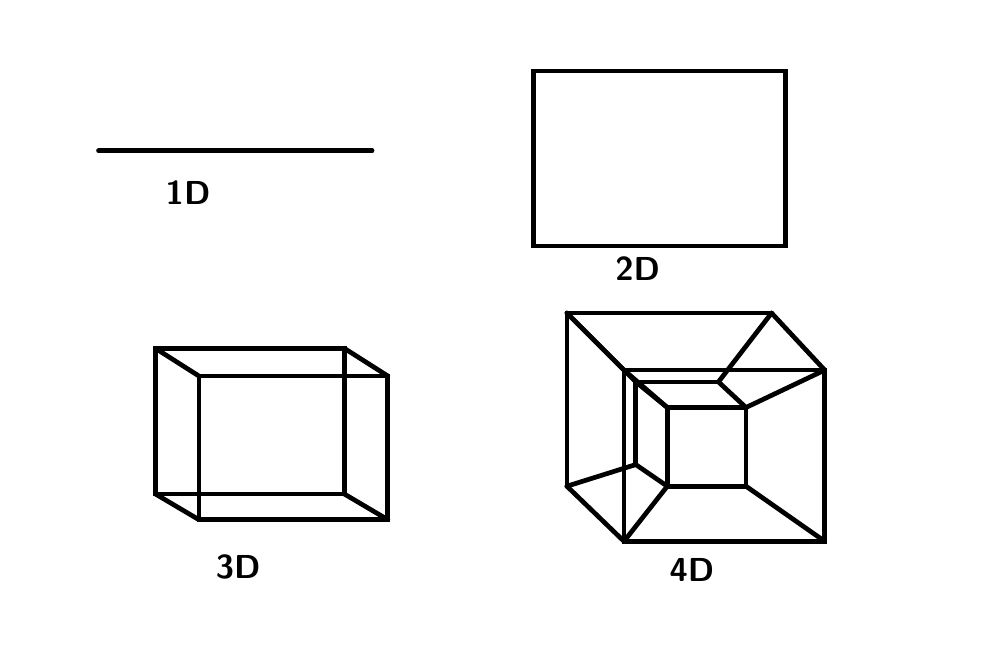
\begin{tikzpicture}[x=0.025cm, y=-0.025cm, line width=1.7pt, line cap=round,
                    lbl/.style={font=\fontsize{12}{12}\selectfont\sffamily\bfseries, inner sep=0pt}]

% full original canvas, including its (asymmetric) margins
\useasboundingbox (0,0) rectangle (482,305);

% ---- 1D: line ----
\draw (36,62.5) -- (175,62.5);
\node[lbl] at (81.5,84) {1D};

% ---- 2D: rectangle ----
\draw (257,22) rectangle (385,111);
\node[lbl] at (310,122.5) {2D};

% ---- 3D: cube (full wireframe, back face up-left) ----
\draw (65,163) rectangle (161,237);   % back face
\draw (87,177) rectangle (183,250);   % front face
\draw (65,163) -- (87,177)  (161,163) -- (183,177)
      (65,237) -- (87,250)  (161,237) -- (183,250);
\node[lbl] at (107,274) {3D};

% ---- 4D: tesseract (outer + inner cube, hidden lines removed) ----
% outer cube: front face A1..A4, back face B1(TL) B2(TR) B4(BL); B3 hidden
\coordinate (A1) at (303,174); \coordinate (A2) at (405,174);
\coordinate (A3) at (405,261); \coordinate (A4) at (303,261);
\coordinate (B1) at (274,145); \coordinate (B2) at (378,145);
\coordinate (B4) at (274,233);
% inner cube: front face a1..a4, back face b1(TL) b2(TR) b4(BL); b3 hidden
\coordinate (a1) at (325,193); \coordinate (a2) at (365,193);
\coordinate (a3) at (365,233); \coordinate (a4) at (325,233);
\coordinate (b1) at (309,180); \coordinate (b2) at (351,180);
\coordinate (b4) at (309,222);

\draw (A1) rectangle (A3);            % outer front face
\draw (B2) -- (B1) -- (B4);           % outer back face: top + left edges only
\draw (B1) -- (A1) (B2) -- (A2) (B4) -- (A4);   % outer corner edges
\draw (a1) rectangle (a3);            % inner front face
\draw (b2) -- (b1) -- (b4);           % inner back face: top + left edges only
\draw (b1) -- (a1) (b2) -- (a2) (b4) -- (a4);   % inner corner edges
% tesseract connectors, outer vertex -> inner vertex
\draw (B1) -- (b1) (B2) -- (b2) (B4) -- (b4)
      (A1) -- (a1) (A2) -- (a2) (A3) -- (a3) (A4) -- (a4);
\node[lbl] at (337.5,275.5) {4D};

\end{tikzpicture}
\end{document}
"
%   mv 1D-4D.pdf ../../images/
%
%   # high-res sRGB PNG (600 dpi) — used in the HTML book
%   xelatex -jobname 1D-4D-rgb "% Source for images/1D-4D.{pdf,png} — geometrical objects in 1 to 4 dimensions,
% shown in 01-Prelude.qmd (chunk `fig-1D-4D`).
%
% This is an author redraw (2026-07-10) of the former low-res raster, which was
% an unattributed web graphic (~98 effective dpi in print; see
% issues/CMYK-checklist.md and issues/fig-permission-list.md). Every coordinate
% is in the original raster's pixel units (482x305 canvas, y down), extracted
% programmatically from the image, so geometry and layout replicate it exactly.
% The tesseract uses hidden-line style, as in the original: the outer and inner
% back faces show only their top and left edges, with no corner edge or
% connector at the hidden back-bottom-right vertex.
%
% Not built by make-diagrams.sh (that script handles the part-page and
% chapter-opener mindmaps only). Rebuild both outputs from this directory:
%
%   # vector PDF, CMYK colors — used in the print/PDF book
%   xelatex -jobname 1D-4D "\def\cmykcolors{}% Source for images/1D-4D.{pdf,png} — geometrical objects in 1 to 4 dimensions,
% shown in 01-Prelude.qmd (chunk `fig-1D-4D`).
%
% This is an author redraw (2026-07-10) of the former low-res raster, which was
% an unattributed web graphic (~98 effective dpi in print; see
% issues/CMYK-checklist.md and issues/fig-permission-list.md). Every coordinate
% is in the original raster's pixel units (482x305 canvas, y down), extracted
% programmatically from the image, so geometry and layout replicate it exactly.
% The tesseract uses hidden-line style, as in the original: the outer and inner
% back faces show only their top and left edges, with no corner edge or
% connector at the hidden back-bottom-right vertex.
%
% Not built by make-diagrams.sh (that script handles the part-page and
% chapter-opener mindmaps only). Rebuild both outputs from this directory:
%
%   # vector PDF, CMYK colors — used in the print/PDF book
%   xelatex -jobname 1D-4D "\def\cmykcolors{}\input{fig-1D-4D.tex}"
%   mv 1D-4D.pdf ../../images/
%
%   # high-res sRGB PNG (600 dpi) — used in the HTML book
%   xelatex -jobname 1D-4D-rgb "\input{fig-1D-4D.tex}"
%   magick -density 600 1D-4D-rgb.pdf -background white -flatten ../../images/1D-4D.png
%   rm -f 1D-4D-rgb.pdf *.aux *.log
%
% The drawing is pure black, so the CMYK variant prints as 100% K ink.
\ifdefined\cmykcolors
  \PassOptionsToPackage{cmyk}{xcolor}
\else
  \PassOptionsToPackage{rgb}{xcolor}
\fi
\documentclass[border=0pt]{standalone}
\usepackage{fontspec}
\setsansfont{Arial}  % labels match the original raster's Arial; needs xelatex
\usepackage{tikz}

\begin{document}
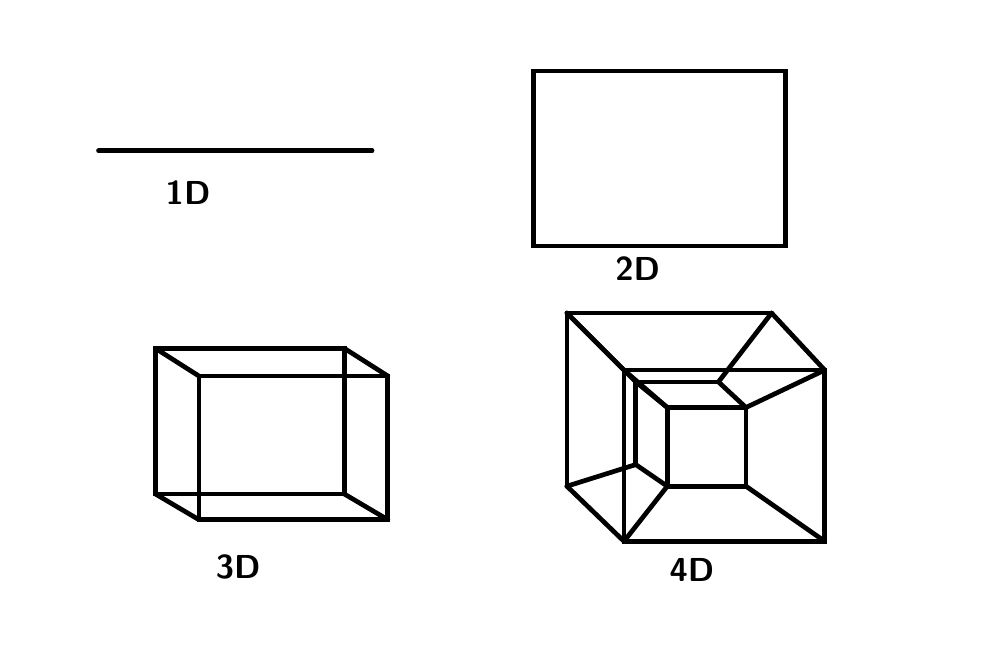
\begin{tikzpicture}[x=0.025cm, y=-0.025cm, line width=1.7pt, line cap=round,
                    lbl/.style={font=\fontsize{12}{12}\selectfont\sffamily\bfseries, inner sep=0pt}]

% full original canvas, including its (asymmetric) margins
\useasboundingbox (0,0) rectangle (482,305);

% ---- 1D: line ----
\draw (36,62.5) -- (175,62.5);
\node[lbl] at (81.5,84) {1D};

% ---- 2D: rectangle ----
\draw (257,22) rectangle (385,111);
\node[lbl] at (310,122.5) {2D};

% ---- 3D: cube (full wireframe, back face up-left) ----
\draw (65,163) rectangle (161,237);   % back face
\draw (87,177) rectangle (183,250);   % front face
\draw (65,163) -- (87,177)  (161,163) -- (183,177)
      (65,237) -- (87,250)  (161,237) -- (183,250);
\node[lbl] at (107,274) {3D};

% ---- 4D: tesseract (outer + inner cube, hidden lines removed) ----
% outer cube: front face A1..A4, back face B1(TL) B2(TR) B4(BL); B3 hidden
\coordinate (A1) at (303,174); \coordinate (A2) at (405,174);
\coordinate (A3) at (405,261); \coordinate (A4) at (303,261);
\coordinate (B1) at (274,145); \coordinate (B2) at (378,145);
\coordinate (B4) at (274,233);
% inner cube: front face a1..a4, back face b1(TL) b2(TR) b4(BL); b3 hidden
\coordinate (a1) at (325,193); \coordinate (a2) at (365,193);
\coordinate (a3) at (365,233); \coordinate (a4) at (325,233);
\coordinate (b1) at (309,180); \coordinate (b2) at (351,180);
\coordinate (b4) at (309,222);

\draw (A1) rectangle (A3);            % outer front face
\draw (B2) -- (B1) -- (B4);           % outer back face: top + left edges only
\draw (B1) -- (A1) (B2) -- (A2) (B4) -- (A4);   % outer corner edges
\draw (a1) rectangle (a3);            % inner front face
\draw (b2) -- (b1) -- (b4);           % inner back face: top + left edges only
\draw (b1) -- (a1) (b2) -- (a2) (b4) -- (a4);   % inner corner edges
% tesseract connectors, outer vertex -> inner vertex
\draw (B1) -- (b1) (B2) -- (b2) (B4) -- (b4)
      (A1) -- (a1) (A2) -- (a2) (A3) -- (a3) (A4) -- (a4);
\node[lbl] at (337.5,275.5) {4D};

\end{tikzpicture}
\end{document}
"
%   mv 1D-4D.pdf ../../images/
%
%   # high-res sRGB PNG (600 dpi) — used in the HTML book
%   xelatex -jobname 1D-4D-rgb "% Source for images/1D-4D.{pdf,png} — geometrical objects in 1 to 4 dimensions,
% shown in 01-Prelude.qmd (chunk `fig-1D-4D`).
%
% This is an author redraw (2026-07-10) of the former low-res raster, which was
% an unattributed web graphic (~98 effective dpi in print; see
% issues/CMYK-checklist.md and issues/fig-permission-list.md). Every coordinate
% is in the original raster's pixel units (482x305 canvas, y down), extracted
% programmatically from the image, so geometry and layout replicate it exactly.
% The tesseract uses hidden-line style, as in the original: the outer and inner
% back faces show only their top and left edges, with no corner edge or
% connector at the hidden back-bottom-right vertex.
%
% Not built by make-diagrams.sh (that script handles the part-page and
% chapter-opener mindmaps only). Rebuild both outputs from this directory:
%
%   # vector PDF, CMYK colors — used in the print/PDF book
%   xelatex -jobname 1D-4D "\def\cmykcolors{}\input{fig-1D-4D.tex}"
%   mv 1D-4D.pdf ../../images/
%
%   # high-res sRGB PNG (600 dpi) — used in the HTML book
%   xelatex -jobname 1D-4D-rgb "\input{fig-1D-4D.tex}"
%   magick -density 600 1D-4D-rgb.pdf -background white -flatten ../../images/1D-4D.png
%   rm -f 1D-4D-rgb.pdf *.aux *.log
%
% The drawing is pure black, so the CMYK variant prints as 100% K ink.
\ifdefined\cmykcolors
  \PassOptionsToPackage{cmyk}{xcolor}
\else
  \PassOptionsToPackage{rgb}{xcolor}
\fi
\documentclass[border=0pt]{standalone}
\usepackage{fontspec}
\setsansfont{Arial}  % labels match the original raster's Arial; needs xelatex
\usepackage{tikz}

\begin{document}
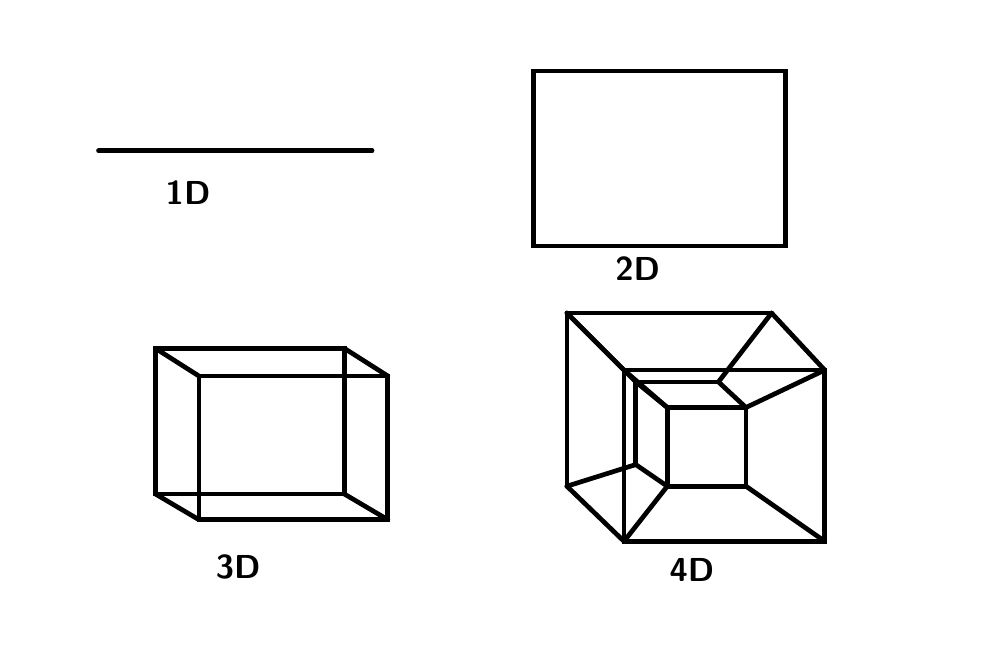
\begin{tikzpicture}[x=0.025cm, y=-0.025cm, line width=1.7pt, line cap=round,
                    lbl/.style={font=\fontsize{12}{12}\selectfont\sffamily\bfseries, inner sep=0pt}]

% full original canvas, including its (asymmetric) margins
\useasboundingbox (0,0) rectangle (482,305);

% ---- 1D: line ----
\draw (36,62.5) -- (175,62.5);
\node[lbl] at (81.5,84) {1D};

% ---- 2D: rectangle ----
\draw (257,22) rectangle (385,111);
\node[lbl] at (310,122.5) {2D};

% ---- 3D: cube (full wireframe, back face up-left) ----
\draw (65,163) rectangle (161,237);   % back face
\draw (87,177) rectangle (183,250);   % front face
\draw (65,163) -- (87,177)  (161,163) -- (183,177)
      (65,237) -- (87,250)  (161,237) -- (183,250);
\node[lbl] at (107,274) {3D};

% ---- 4D: tesseract (outer + inner cube, hidden lines removed) ----
% outer cube: front face A1..A4, back face B1(TL) B2(TR) B4(BL); B3 hidden
\coordinate (A1) at (303,174); \coordinate (A2) at (405,174);
\coordinate (A3) at (405,261); \coordinate (A4) at (303,261);
\coordinate (B1) at (274,145); \coordinate (B2) at (378,145);
\coordinate (B4) at (274,233);
% inner cube: front face a1..a4, back face b1(TL) b2(TR) b4(BL); b3 hidden
\coordinate (a1) at (325,193); \coordinate (a2) at (365,193);
\coordinate (a3) at (365,233); \coordinate (a4) at (325,233);
\coordinate (b1) at (309,180); \coordinate (b2) at (351,180);
\coordinate (b4) at (309,222);

\draw (A1) rectangle (A3);            % outer front face
\draw (B2) -- (B1) -- (B4);           % outer back face: top + left edges only
\draw (B1) -- (A1) (B2) -- (A2) (B4) -- (A4);   % outer corner edges
\draw (a1) rectangle (a3);            % inner front face
\draw (b2) -- (b1) -- (b4);           % inner back face: top + left edges only
\draw (b1) -- (a1) (b2) -- (a2) (b4) -- (a4);   % inner corner edges
% tesseract connectors, outer vertex -> inner vertex
\draw (B1) -- (b1) (B2) -- (b2) (B4) -- (b4)
      (A1) -- (a1) (A2) -- (a2) (A3) -- (a3) (A4) -- (a4);
\node[lbl] at (337.5,275.5) {4D};

\end{tikzpicture}
\end{document}
"
%   magick -density 600 1D-4D-rgb.pdf -background white -flatten ../../images/1D-4D.png
%   rm -f 1D-4D-rgb.pdf *.aux *.log
%
% The drawing is pure black, so the CMYK variant prints as 100% K ink.
\ifdefined\cmykcolors
  \PassOptionsToPackage{cmyk}{xcolor}
\else
  \PassOptionsToPackage{rgb}{xcolor}
\fi
\documentclass[border=0pt]{standalone}
\usepackage{fontspec}
\setsansfont{Arial}  % labels match the original raster's Arial; needs xelatex
\usepackage{tikz}

\begin{document}
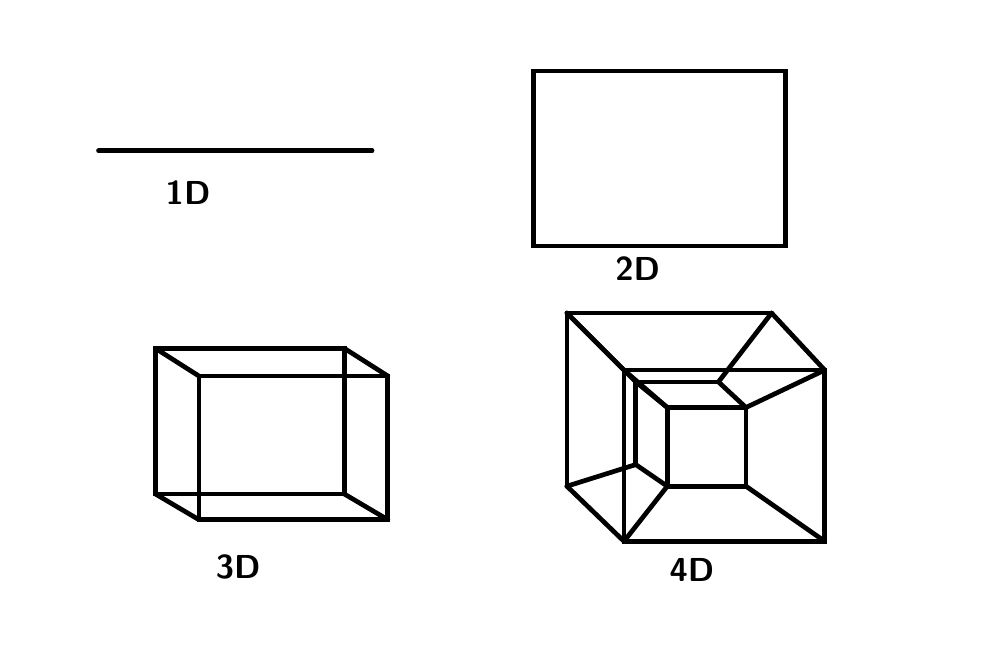
\begin{tikzpicture}[x=0.025cm, y=-0.025cm, line width=1.7pt, line cap=round,
                    lbl/.style={font=\fontsize{12}{12}\selectfont\sffamily\bfseries, inner sep=0pt}]

% full original canvas, including its (asymmetric) margins
\useasboundingbox (0,0) rectangle (482,305);

% ---- 1D: line ----
\draw (36,62.5) -- (175,62.5);
\node[lbl] at (81.5,84) {1D};

% ---- 2D: rectangle ----
\draw (257,22) rectangle (385,111);
\node[lbl] at (310,122.5) {2D};

% ---- 3D: cube (full wireframe, back face up-left) ----
\draw (65,163) rectangle (161,237);   % back face
\draw (87,177) rectangle (183,250);   % front face
\draw (65,163) -- (87,177)  (161,163) -- (183,177)
      (65,237) -- (87,250)  (161,237) -- (183,250);
\node[lbl] at (107,274) {3D};

% ---- 4D: tesseract (outer + inner cube, hidden lines removed) ----
% outer cube: front face A1..A4, back face B1(TL) B2(TR) B4(BL); B3 hidden
\coordinate (A1) at (303,174); \coordinate (A2) at (405,174);
\coordinate (A3) at (405,261); \coordinate (A4) at (303,261);
\coordinate (B1) at (274,145); \coordinate (B2) at (378,145);
\coordinate (B4) at (274,233);
% inner cube: front face a1..a4, back face b1(TL) b2(TR) b4(BL); b3 hidden
\coordinate (a1) at (325,193); \coordinate (a2) at (365,193);
\coordinate (a3) at (365,233); \coordinate (a4) at (325,233);
\coordinate (b1) at (309,180); \coordinate (b2) at (351,180);
\coordinate (b4) at (309,222);

\draw (A1) rectangle (A3);            % outer front face
\draw (B2) -- (B1) -- (B4);           % outer back face: top + left edges only
\draw (B1) -- (A1) (B2) -- (A2) (B4) -- (A4);   % outer corner edges
\draw (a1) rectangle (a3);            % inner front face
\draw (b2) -- (b1) -- (b4);           % inner back face: top + left edges only
\draw (b1) -- (a1) (b2) -- (a2) (b4) -- (a4);   % inner corner edges
% tesseract connectors, outer vertex -> inner vertex
\draw (B1) -- (b1) (B2) -- (b2) (B4) -- (b4)
      (A1) -- (a1) (A2) -- (a2) (A3) -- (a3) (A4) -- (a4);
\node[lbl] at (337.5,275.5) {4D};

\end{tikzpicture}
\end{document}
"
%   magick -density 600 1D-4D-rgb.pdf -background white -flatten ../../images/1D-4D.png
%   rm -f 1D-4D-rgb.pdf *.aux *.log
%
% The drawing is pure black, so the CMYK variant prints as 100% K ink.
\ifdefined\cmykcolors
  \PassOptionsToPackage{cmyk}{xcolor}
\else
  \PassOptionsToPackage{rgb}{xcolor}
\fi
\documentclass[border=0pt]{standalone}
\usepackage{fontspec}
\setsansfont{Arial}  % labels match the original raster's Arial; needs xelatex
\usepackage{tikz}

\begin{document}
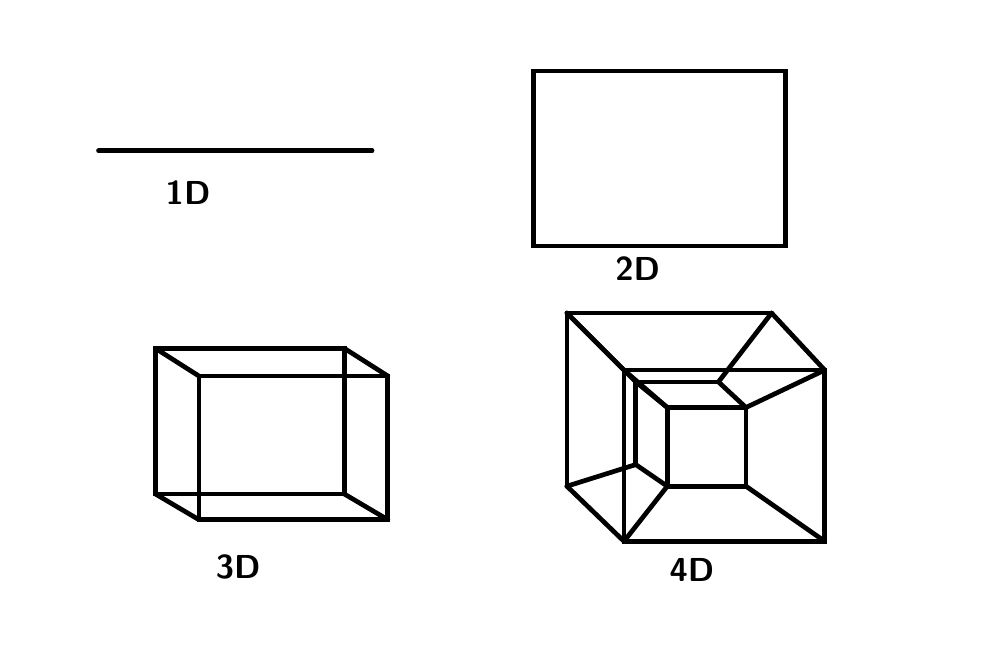
\begin{tikzpicture}[x=0.025cm, y=-0.025cm, line width=1.7pt, line cap=round,
                    lbl/.style={font=\fontsize{12}{12}\selectfont\sffamily\bfseries, inner sep=0pt}]

% full original canvas, including its (asymmetric) margins
\useasboundingbox (0,0) rectangle (482,305);

% ---- 1D: line ----
\draw (36,62.5) -- (175,62.5);
\node[lbl] at (81.5,84) {1D};

% ---- 2D: rectangle ----
\draw (257,22) rectangle (385,111);
\node[lbl] at (310,122.5) {2D};

% ---- 3D: cube (full wireframe, back face up-left) ----
\draw (65,163) rectangle (161,237);   % back face
\draw (87,177) rectangle (183,250);   % front face
\draw (65,163) -- (87,177)  (161,163) -- (183,177)
      (65,237) -- (87,250)  (161,237) -- (183,250);
\node[lbl] at (107,274) {3D};

% ---- 4D: tesseract (outer + inner cube, hidden lines removed) ----
% outer cube: front face A1..A4, back face B1(TL) B2(TR) B4(BL); B3 hidden
\coordinate (A1) at (303,174); \coordinate (A2) at (405,174);
\coordinate (A3) at (405,261); \coordinate (A4) at (303,261);
\coordinate (B1) at (274,145); \coordinate (B2) at (378,145);
\coordinate (B4) at (274,233);
% inner cube: front face a1..a4, back face b1(TL) b2(TR) b4(BL); b3 hidden
\coordinate (a1) at (325,193); \coordinate (a2) at (365,193);
\coordinate (a3) at (365,233); \coordinate (a4) at (325,233);
\coordinate (b1) at (309,180); \coordinate (b2) at (351,180);
\coordinate (b4) at (309,222);

\draw (A1) rectangle (A3);            % outer front face
\draw (B2) -- (B1) -- (B4);           % outer back face: top + left edges only
\draw (B1) -- (A1) (B2) -- (A2) (B4) -- (A4);   % outer corner edges
\draw (a1) rectangle (a3);            % inner front face
\draw (b2) -- (b1) -- (b4);           % inner back face: top + left edges only
\draw (b1) -- (a1) (b2) -- (a2) (b4) -- (a4);   % inner corner edges
% tesseract connectors, outer vertex -> inner vertex
\draw (B1) -- (b1) (B2) -- (b2) (B4) -- (b4)
      (A1) -- (a1) (A2) -- (a2) (A3) -- (a3) (A4) -- (a4);
\node[lbl] at (337.5,275.5) {4D};

\end{tikzpicture}
\end{document}
"
%   mv 1D-4D.pdf ../../images/
%
%   # high-res sRGB PNG (600 dpi) — used in the HTML book
%   xelatex -jobname 1D-4D-rgb "% Source for images/1D-4D.{pdf,png} — geometrical objects in 1 to 4 dimensions,
% shown in 01-Prelude.qmd (chunk `fig-1D-4D`).
%
% This is an author redraw (2026-07-10) of the former low-res raster, which was
% an unattributed web graphic (~98 effective dpi in print; see
% issues/CMYK-checklist.md and issues/fig-permission-list.md). Every coordinate
% is in the original raster's pixel units (482x305 canvas, y down), extracted
% programmatically from the image, so geometry and layout replicate it exactly.
% The tesseract uses hidden-line style, as in the original: the outer and inner
% back faces show only their top and left edges, with no corner edge or
% connector at the hidden back-bottom-right vertex.
%
% Not built by make-diagrams.sh (that script handles the part-page and
% chapter-opener mindmaps only). Rebuild both outputs from this directory:
%
%   # vector PDF, CMYK colors — used in the print/PDF book
%   xelatex -jobname 1D-4D "\def\cmykcolors{}% Source for images/1D-4D.{pdf,png} — geometrical objects in 1 to 4 dimensions,
% shown in 01-Prelude.qmd (chunk `fig-1D-4D`).
%
% This is an author redraw (2026-07-10) of the former low-res raster, which was
% an unattributed web graphic (~98 effective dpi in print; see
% issues/CMYK-checklist.md and issues/fig-permission-list.md). Every coordinate
% is in the original raster's pixel units (482x305 canvas, y down), extracted
% programmatically from the image, so geometry and layout replicate it exactly.
% The tesseract uses hidden-line style, as in the original: the outer and inner
% back faces show only their top and left edges, with no corner edge or
% connector at the hidden back-bottom-right vertex.
%
% Not built by make-diagrams.sh (that script handles the part-page and
% chapter-opener mindmaps only). Rebuild both outputs from this directory:
%
%   # vector PDF, CMYK colors — used in the print/PDF book
%   xelatex -jobname 1D-4D "\def\cmykcolors{}% Source for images/1D-4D.{pdf,png} — geometrical objects in 1 to 4 dimensions,
% shown in 01-Prelude.qmd (chunk `fig-1D-4D`).
%
% This is an author redraw (2026-07-10) of the former low-res raster, which was
% an unattributed web graphic (~98 effective dpi in print; see
% issues/CMYK-checklist.md and issues/fig-permission-list.md). Every coordinate
% is in the original raster's pixel units (482x305 canvas, y down), extracted
% programmatically from the image, so geometry and layout replicate it exactly.
% The tesseract uses hidden-line style, as in the original: the outer and inner
% back faces show only their top and left edges, with no corner edge or
% connector at the hidden back-bottom-right vertex.
%
% Not built by make-diagrams.sh (that script handles the part-page and
% chapter-opener mindmaps only). Rebuild both outputs from this directory:
%
%   # vector PDF, CMYK colors — used in the print/PDF book
%   xelatex -jobname 1D-4D "\def\cmykcolors{}\input{fig-1D-4D.tex}"
%   mv 1D-4D.pdf ../../images/
%
%   # high-res sRGB PNG (600 dpi) — used in the HTML book
%   xelatex -jobname 1D-4D-rgb "\input{fig-1D-4D.tex}"
%   magick -density 600 1D-4D-rgb.pdf -background white -flatten ../../images/1D-4D.png
%   rm -f 1D-4D-rgb.pdf *.aux *.log
%
% The drawing is pure black, so the CMYK variant prints as 100% K ink.
\ifdefined\cmykcolors
  \PassOptionsToPackage{cmyk}{xcolor}
\else
  \PassOptionsToPackage{rgb}{xcolor}
\fi
\documentclass[border=0pt]{standalone}
\usepackage{fontspec}
\setsansfont{Arial}  % labels match the original raster's Arial; needs xelatex
\usepackage{tikz}

\begin{document}
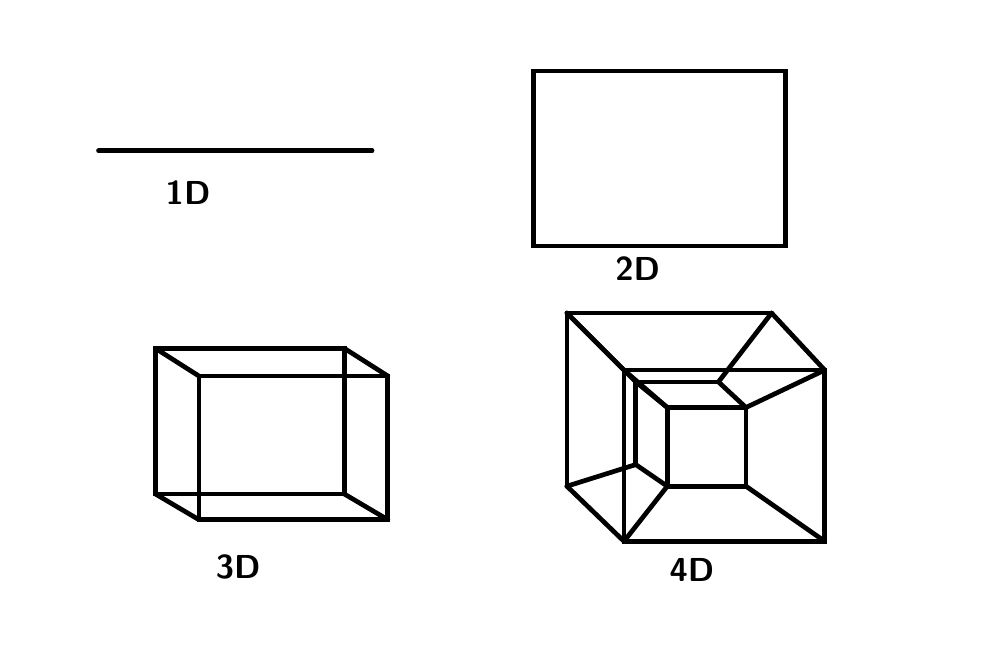
\begin{tikzpicture}[x=0.025cm, y=-0.025cm, line width=1.7pt, line cap=round,
                    lbl/.style={font=\fontsize{12}{12}\selectfont\sffamily\bfseries, inner sep=0pt}]

% full original canvas, including its (asymmetric) margins
\useasboundingbox (0,0) rectangle (482,305);

% ---- 1D: line ----
\draw (36,62.5) -- (175,62.5);
\node[lbl] at (81.5,84) {1D};

% ---- 2D: rectangle ----
\draw (257,22) rectangle (385,111);
\node[lbl] at (310,122.5) {2D};

% ---- 3D: cube (full wireframe, back face up-left) ----
\draw (65,163) rectangle (161,237);   % back face
\draw (87,177) rectangle (183,250);   % front face
\draw (65,163) -- (87,177)  (161,163) -- (183,177)
      (65,237) -- (87,250)  (161,237) -- (183,250);
\node[lbl] at (107,274) {3D};

% ---- 4D: tesseract (outer + inner cube, hidden lines removed) ----
% outer cube: front face A1..A4, back face B1(TL) B2(TR) B4(BL); B3 hidden
\coordinate (A1) at (303,174); \coordinate (A2) at (405,174);
\coordinate (A3) at (405,261); \coordinate (A4) at (303,261);
\coordinate (B1) at (274,145); \coordinate (B2) at (378,145);
\coordinate (B4) at (274,233);
% inner cube: front face a1..a4, back face b1(TL) b2(TR) b4(BL); b3 hidden
\coordinate (a1) at (325,193); \coordinate (a2) at (365,193);
\coordinate (a3) at (365,233); \coordinate (a4) at (325,233);
\coordinate (b1) at (309,180); \coordinate (b2) at (351,180);
\coordinate (b4) at (309,222);

\draw (A1) rectangle (A3);            % outer front face
\draw (B2) -- (B1) -- (B4);           % outer back face: top + left edges only
\draw (B1) -- (A1) (B2) -- (A2) (B4) -- (A4);   % outer corner edges
\draw (a1) rectangle (a3);            % inner front face
\draw (b2) -- (b1) -- (b4);           % inner back face: top + left edges only
\draw (b1) -- (a1) (b2) -- (a2) (b4) -- (a4);   % inner corner edges
% tesseract connectors, outer vertex -> inner vertex
\draw (B1) -- (b1) (B2) -- (b2) (B4) -- (b4)
      (A1) -- (a1) (A2) -- (a2) (A3) -- (a3) (A4) -- (a4);
\node[lbl] at (337.5,275.5) {4D};

\end{tikzpicture}
\end{document}
"
%   mv 1D-4D.pdf ../../images/
%
%   # high-res sRGB PNG (600 dpi) — used in the HTML book
%   xelatex -jobname 1D-4D-rgb "% Source for images/1D-4D.{pdf,png} — geometrical objects in 1 to 4 dimensions,
% shown in 01-Prelude.qmd (chunk `fig-1D-4D`).
%
% This is an author redraw (2026-07-10) of the former low-res raster, which was
% an unattributed web graphic (~98 effective dpi in print; see
% issues/CMYK-checklist.md and issues/fig-permission-list.md). Every coordinate
% is in the original raster's pixel units (482x305 canvas, y down), extracted
% programmatically from the image, so geometry and layout replicate it exactly.
% The tesseract uses hidden-line style, as in the original: the outer and inner
% back faces show only their top and left edges, with no corner edge or
% connector at the hidden back-bottom-right vertex.
%
% Not built by make-diagrams.sh (that script handles the part-page and
% chapter-opener mindmaps only). Rebuild both outputs from this directory:
%
%   # vector PDF, CMYK colors — used in the print/PDF book
%   xelatex -jobname 1D-4D "\def\cmykcolors{}\input{fig-1D-4D.tex}"
%   mv 1D-4D.pdf ../../images/
%
%   # high-res sRGB PNG (600 dpi) — used in the HTML book
%   xelatex -jobname 1D-4D-rgb "\input{fig-1D-4D.tex}"
%   magick -density 600 1D-4D-rgb.pdf -background white -flatten ../../images/1D-4D.png
%   rm -f 1D-4D-rgb.pdf *.aux *.log
%
% The drawing is pure black, so the CMYK variant prints as 100% K ink.
\ifdefined\cmykcolors
  \PassOptionsToPackage{cmyk}{xcolor}
\else
  \PassOptionsToPackage{rgb}{xcolor}
\fi
\documentclass[border=0pt]{standalone}
\usepackage{fontspec}
\setsansfont{Arial}  % labels match the original raster's Arial; needs xelatex
\usepackage{tikz}

\begin{document}
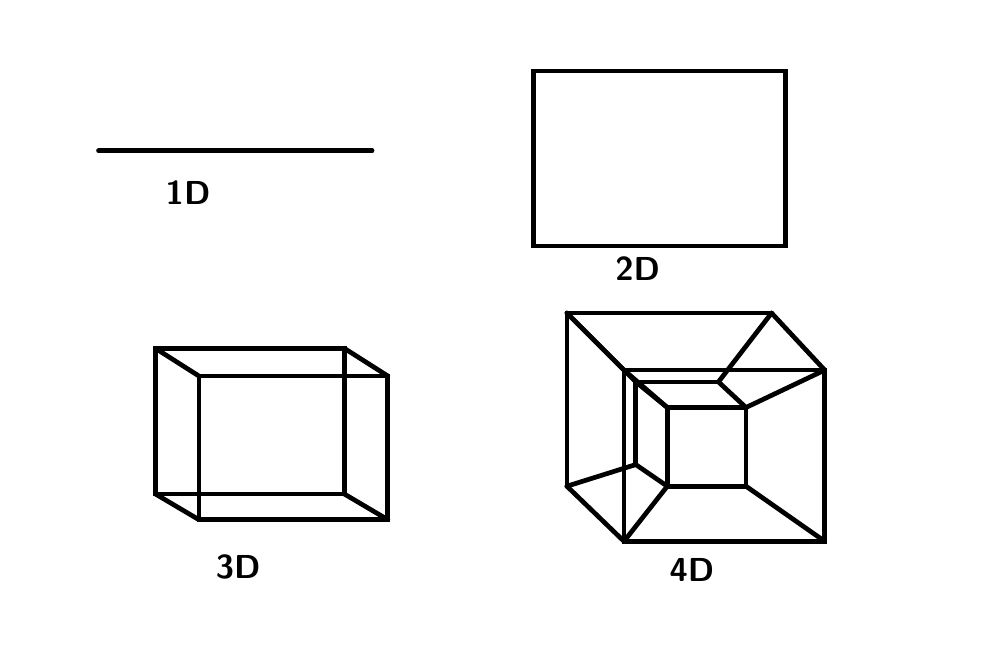
\begin{tikzpicture}[x=0.025cm, y=-0.025cm, line width=1.7pt, line cap=round,
                    lbl/.style={font=\fontsize{12}{12}\selectfont\sffamily\bfseries, inner sep=0pt}]

% full original canvas, including its (asymmetric) margins
\useasboundingbox (0,0) rectangle (482,305);

% ---- 1D: line ----
\draw (36,62.5) -- (175,62.5);
\node[lbl] at (81.5,84) {1D};

% ---- 2D: rectangle ----
\draw (257,22) rectangle (385,111);
\node[lbl] at (310,122.5) {2D};

% ---- 3D: cube (full wireframe, back face up-left) ----
\draw (65,163) rectangle (161,237);   % back face
\draw (87,177) rectangle (183,250);   % front face
\draw (65,163) -- (87,177)  (161,163) -- (183,177)
      (65,237) -- (87,250)  (161,237) -- (183,250);
\node[lbl] at (107,274) {3D};

% ---- 4D: tesseract (outer + inner cube, hidden lines removed) ----
% outer cube: front face A1..A4, back face B1(TL) B2(TR) B4(BL); B3 hidden
\coordinate (A1) at (303,174); \coordinate (A2) at (405,174);
\coordinate (A3) at (405,261); \coordinate (A4) at (303,261);
\coordinate (B1) at (274,145); \coordinate (B2) at (378,145);
\coordinate (B4) at (274,233);
% inner cube: front face a1..a4, back face b1(TL) b2(TR) b4(BL); b3 hidden
\coordinate (a1) at (325,193); \coordinate (a2) at (365,193);
\coordinate (a3) at (365,233); \coordinate (a4) at (325,233);
\coordinate (b1) at (309,180); \coordinate (b2) at (351,180);
\coordinate (b4) at (309,222);

\draw (A1) rectangle (A3);            % outer front face
\draw (B2) -- (B1) -- (B4);           % outer back face: top + left edges only
\draw (B1) -- (A1) (B2) -- (A2) (B4) -- (A4);   % outer corner edges
\draw (a1) rectangle (a3);            % inner front face
\draw (b2) -- (b1) -- (b4);           % inner back face: top + left edges only
\draw (b1) -- (a1) (b2) -- (a2) (b4) -- (a4);   % inner corner edges
% tesseract connectors, outer vertex -> inner vertex
\draw (B1) -- (b1) (B2) -- (b2) (B4) -- (b4)
      (A1) -- (a1) (A2) -- (a2) (A3) -- (a3) (A4) -- (a4);
\node[lbl] at (337.5,275.5) {4D};

\end{tikzpicture}
\end{document}
"
%   magick -density 600 1D-4D-rgb.pdf -background white -flatten ../../images/1D-4D.png
%   rm -f 1D-4D-rgb.pdf *.aux *.log
%
% The drawing is pure black, so the CMYK variant prints as 100% K ink.
\ifdefined\cmykcolors
  \PassOptionsToPackage{cmyk}{xcolor}
\else
  \PassOptionsToPackage{rgb}{xcolor}
\fi
\documentclass[border=0pt]{standalone}
\usepackage{fontspec}
\setsansfont{Arial}  % labels match the original raster's Arial; needs xelatex
\usepackage{tikz}

\begin{document}
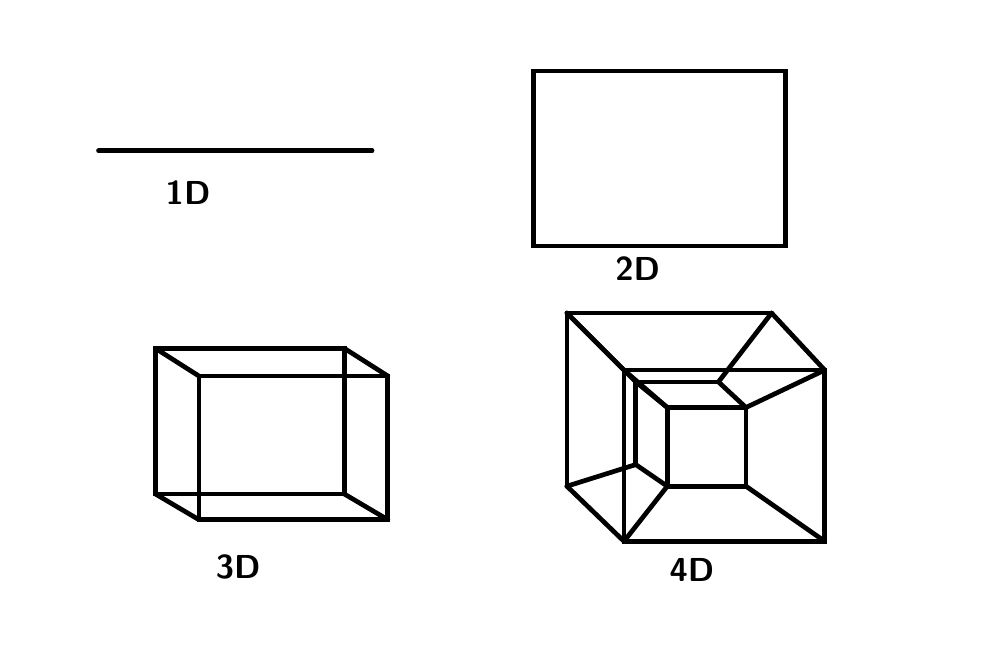
\begin{tikzpicture}[x=0.025cm, y=-0.025cm, line width=1.7pt, line cap=round,
                    lbl/.style={font=\fontsize{12}{12}\selectfont\sffamily\bfseries, inner sep=0pt}]

% full original canvas, including its (asymmetric) margins
\useasboundingbox (0,0) rectangle (482,305);

% ---- 1D: line ----
\draw (36,62.5) -- (175,62.5);
\node[lbl] at (81.5,84) {1D};

% ---- 2D: rectangle ----
\draw (257,22) rectangle (385,111);
\node[lbl] at (310,122.5) {2D};

% ---- 3D: cube (full wireframe, back face up-left) ----
\draw (65,163) rectangle (161,237);   % back face
\draw (87,177) rectangle (183,250);   % front face
\draw (65,163) -- (87,177)  (161,163) -- (183,177)
      (65,237) -- (87,250)  (161,237) -- (183,250);
\node[lbl] at (107,274) {3D};

% ---- 4D: tesseract (outer + inner cube, hidden lines removed) ----
% outer cube: front face A1..A4, back face B1(TL) B2(TR) B4(BL); B3 hidden
\coordinate (A1) at (303,174); \coordinate (A2) at (405,174);
\coordinate (A3) at (405,261); \coordinate (A4) at (303,261);
\coordinate (B1) at (274,145); \coordinate (B2) at (378,145);
\coordinate (B4) at (274,233);
% inner cube: front face a1..a4, back face b1(TL) b2(TR) b4(BL); b3 hidden
\coordinate (a1) at (325,193); \coordinate (a2) at (365,193);
\coordinate (a3) at (365,233); \coordinate (a4) at (325,233);
\coordinate (b1) at (309,180); \coordinate (b2) at (351,180);
\coordinate (b4) at (309,222);

\draw (A1) rectangle (A3);            % outer front face
\draw (B2) -- (B1) -- (B4);           % outer back face: top + left edges only
\draw (B1) -- (A1) (B2) -- (A2) (B4) -- (A4);   % outer corner edges
\draw (a1) rectangle (a3);            % inner front face
\draw (b2) -- (b1) -- (b4);           % inner back face: top + left edges only
\draw (b1) -- (a1) (b2) -- (a2) (b4) -- (a4);   % inner corner edges
% tesseract connectors, outer vertex -> inner vertex
\draw (B1) -- (b1) (B2) -- (b2) (B4) -- (b4)
      (A1) -- (a1) (A2) -- (a2) (A3) -- (a3) (A4) -- (a4);
\node[lbl] at (337.5,275.5) {4D};

\end{tikzpicture}
\end{document}
"
%   mv 1D-4D.pdf ../../images/
%
%   # high-res sRGB PNG (600 dpi) — used in the HTML book
%   xelatex -jobname 1D-4D-rgb "% Source for images/1D-4D.{pdf,png} — geometrical objects in 1 to 4 dimensions,
% shown in 01-Prelude.qmd (chunk `fig-1D-4D`).
%
% This is an author redraw (2026-07-10) of the former low-res raster, which was
% an unattributed web graphic (~98 effective dpi in print; see
% issues/CMYK-checklist.md and issues/fig-permission-list.md). Every coordinate
% is in the original raster's pixel units (482x305 canvas, y down), extracted
% programmatically from the image, so geometry and layout replicate it exactly.
% The tesseract uses hidden-line style, as in the original: the outer and inner
% back faces show only their top and left edges, with no corner edge or
% connector at the hidden back-bottom-right vertex.
%
% Not built by make-diagrams.sh (that script handles the part-page and
% chapter-opener mindmaps only). Rebuild both outputs from this directory:
%
%   # vector PDF, CMYK colors — used in the print/PDF book
%   xelatex -jobname 1D-4D "\def\cmykcolors{}% Source for images/1D-4D.{pdf,png} — geometrical objects in 1 to 4 dimensions,
% shown in 01-Prelude.qmd (chunk `fig-1D-4D`).
%
% This is an author redraw (2026-07-10) of the former low-res raster, which was
% an unattributed web graphic (~98 effective dpi in print; see
% issues/CMYK-checklist.md and issues/fig-permission-list.md). Every coordinate
% is in the original raster's pixel units (482x305 canvas, y down), extracted
% programmatically from the image, so geometry and layout replicate it exactly.
% The tesseract uses hidden-line style, as in the original: the outer and inner
% back faces show only their top and left edges, with no corner edge or
% connector at the hidden back-bottom-right vertex.
%
% Not built by make-diagrams.sh (that script handles the part-page and
% chapter-opener mindmaps only). Rebuild both outputs from this directory:
%
%   # vector PDF, CMYK colors — used in the print/PDF book
%   xelatex -jobname 1D-4D "\def\cmykcolors{}\input{fig-1D-4D.tex}"
%   mv 1D-4D.pdf ../../images/
%
%   # high-res sRGB PNG (600 dpi) — used in the HTML book
%   xelatex -jobname 1D-4D-rgb "\input{fig-1D-4D.tex}"
%   magick -density 600 1D-4D-rgb.pdf -background white -flatten ../../images/1D-4D.png
%   rm -f 1D-4D-rgb.pdf *.aux *.log
%
% The drawing is pure black, so the CMYK variant prints as 100% K ink.
\ifdefined\cmykcolors
  \PassOptionsToPackage{cmyk}{xcolor}
\else
  \PassOptionsToPackage{rgb}{xcolor}
\fi
\documentclass[border=0pt]{standalone}
\usepackage{fontspec}
\setsansfont{Arial}  % labels match the original raster's Arial; needs xelatex
\usepackage{tikz}

\begin{document}
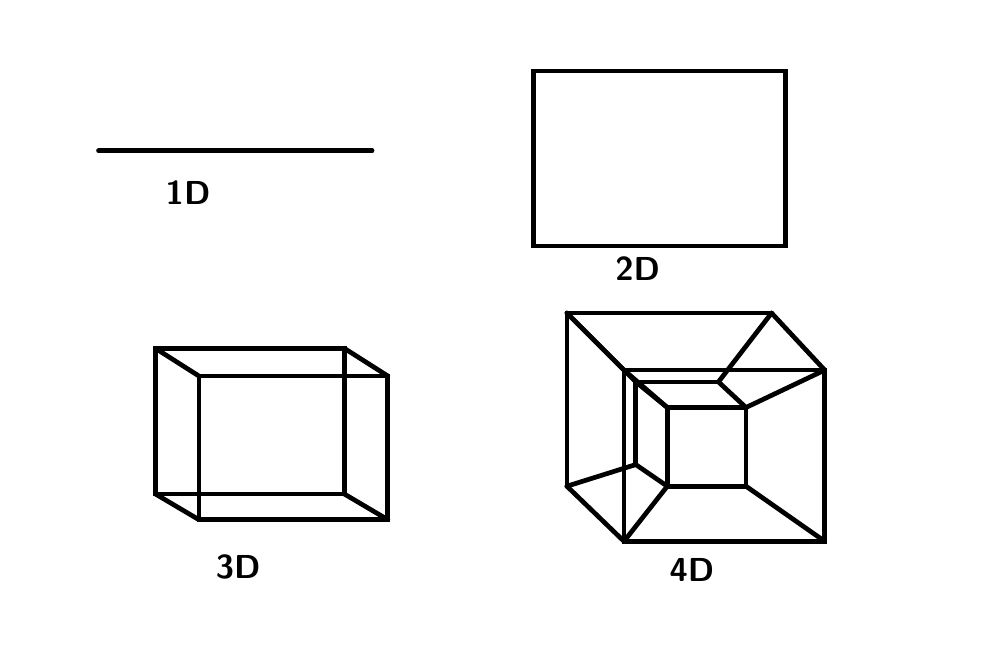
\begin{tikzpicture}[x=0.025cm, y=-0.025cm, line width=1.7pt, line cap=round,
                    lbl/.style={font=\fontsize{12}{12}\selectfont\sffamily\bfseries, inner sep=0pt}]

% full original canvas, including its (asymmetric) margins
\useasboundingbox (0,0) rectangle (482,305);

% ---- 1D: line ----
\draw (36,62.5) -- (175,62.5);
\node[lbl] at (81.5,84) {1D};

% ---- 2D: rectangle ----
\draw (257,22) rectangle (385,111);
\node[lbl] at (310,122.5) {2D};

% ---- 3D: cube (full wireframe, back face up-left) ----
\draw (65,163) rectangle (161,237);   % back face
\draw (87,177) rectangle (183,250);   % front face
\draw (65,163) -- (87,177)  (161,163) -- (183,177)
      (65,237) -- (87,250)  (161,237) -- (183,250);
\node[lbl] at (107,274) {3D};

% ---- 4D: tesseract (outer + inner cube, hidden lines removed) ----
% outer cube: front face A1..A4, back face B1(TL) B2(TR) B4(BL); B3 hidden
\coordinate (A1) at (303,174); \coordinate (A2) at (405,174);
\coordinate (A3) at (405,261); \coordinate (A4) at (303,261);
\coordinate (B1) at (274,145); \coordinate (B2) at (378,145);
\coordinate (B4) at (274,233);
% inner cube: front face a1..a4, back face b1(TL) b2(TR) b4(BL); b3 hidden
\coordinate (a1) at (325,193); \coordinate (a2) at (365,193);
\coordinate (a3) at (365,233); \coordinate (a4) at (325,233);
\coordinate (b1) at (309,180); \coordinate (b2) at (351,180);
\coordinate (b4) at (309,222);

\draw (A1) rectangle (A3);            % outer front face
\draw (B2) -- (B1) -- (B4);           % outer back face: top + left edges only
\draw (B1) -- (A1) (B2) -- (A2) (B4) -- (A4);   % outer corner edges
\draw (a1) rectangle (a3);            % inner front face
\draw (b2) -- (b1) -- (b4);           % inner back face: top + left edges only
\draw (b1) -- (a1) (b2) -- (a2) (b4) -- (a4);   % inner corner edges
% tesseract connectors, outer vertex -> inner vertex
\draw (B1) -- (b1) (B2) -- (b2) (B4) -- (b4)
      (A1) -- (a1) (A2) -- (a2) (A3) -- (a3) (A4) -- (a4);
\node[lbl] at (337.5,275.5) {4D};

\end{tikzpicture}
\end{document}
"
%   mv 1D-4D.pdf ../../images/
%
%   # high-res sRGB PNG (600 dpi) — used in the HTML book
%   xelatex -jobname 1D-4D-rgb "% Source for images/1D-4D.{pdf,png} — geometrical objects in 1 to 4 dimensions,
% shown in 01-Prelude.qmd (chunk `fig-1D-4D`).
%
% This is an author redraw (2026-07-10) of the former low-res raster, which was
% an unattributed web graphic (~98 effective dpi in print; see
% issues/CMYK-checklist.md and issues/fig-permission-list.md). Every coordinate
% is in the original raster's pixel units (482x305 canvas, y down), extracted
% programmatically from the image, so geometry and layout replicate it exactly.
% The tesseract uses hidden-line style, as in the original: the outer and inner
% back faces show only their top and left edges, with no corner edge or
% connector at the hidden back-bottom-right vertex.
%
% Not built by make-diagrams.sh (that script handles the part-page and
% chapter-opener mindmaps only). Rebuild both outputs from this directory:
%
%   # vector PDF, CMYK colors — used in the print/PDF book
%   xelatex -jobname 1D-4D "\def\cmykcolors{}\input{fig-1D-4D.tex}"
%   mv 1D-4D.pdf ../../images/
%
%   # high-res sRGB PNG (600 dpi) — used in the HTML book
%   xelatex -jobname 1D-4D-rgb "\input{fig-1D-4D.tex}"
%   magick -density 600 1D-4D-rgb.pdf -background white -flatten ../../images/1D-4D.png
%   rm -f 1D-4D-rgb.pdf *.aux *.log
%
% The drawing is pure black, so the CMYK variant prints as 100% K ink.
\ifdefined\cmykcolors
  \PassOptionsToPackage{cmyk}{xcolor}
\else
  \PassOptionsToPackage{rgb}{xcolor}
\fi
\documentclass[border=0pt]{standalone}
\usepackage{fontspec}
\setsansfont{Arial}  % labels match the original raster's Arial; needs xelatex
\usepackage{tikz}

\begin{document}
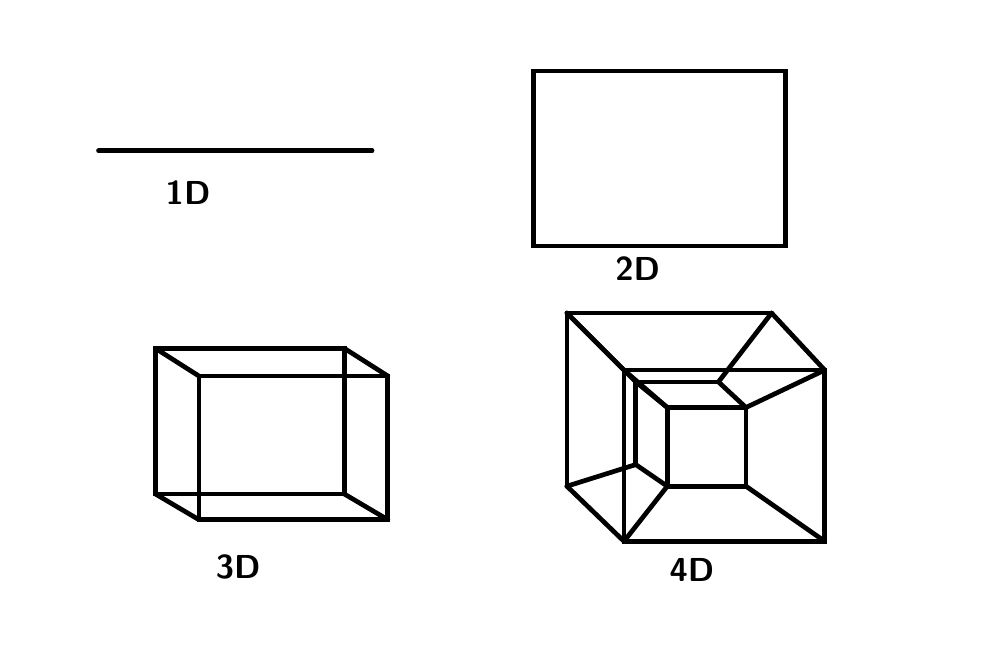
\begin{tikzpicture}[x=0.025cm, y=-0.025cm, line width=1.7pt, line cap=round,
                    lbl/.style={font=\fontsize{12}{12}\selectfont\sffamily\bfseries, inner sep=0pt}]

% full original canvas, including its (asymmetric) margins
\useasboundingbox (0,0) rectangle (482,305);

% ---- 1D: line ----
\draw (36,62.5) -- (175,62.5);
\node[lbl] at (81.5,84) {1D};

% ---- 2D: rectangle ----
\draw (257,22) rectangle (385,111);
\node[lbl] at (310,122.5) {2D};

% ---- 3D: cube (full wireframe, back face up-left) ----
\draw (65,163) rectangle (161,237);   % back face
\draw (87,177) rectangle (183,250);   % front face
\draw (65,163) -- (87,177)  (161,163) -- (183,177)
      (65,237) -- (87,250)  (161,237) -- (183,250);
\node[lbl] at (107,274) {3D};

% ---- 4D: tesseract (outer + inner cube, hidden lines removed) ----
% outer cube: front face A1..A4, back face B1(TL) B2(TR) B4(BL); B3 hidden
\coordinate (A1) at (303,174); \coordinate (A2) at (405,174);
\coordinate (A3) at (405,261); \coordinate (A4) at (303,261);
\coordinate (B1) at (274,145); \coordinate (B2) at (378,145);
\coordinate (B4) at (274,233);
% inner cube: front face a1..a4, back face b1(TL) b2(TR) b4(BL); b3 hidden
\coordinate (a1) at (325,193); \coordinate (a2) at (365,193);
\coordinate (a3) at (365,233); \coordinate (a4) at (325,233);
\coordinate (b1) at (309,180); \coordinate (b2) at (351,180);
\coordinate (b4) at (309,222);

\draw (A1) rectangle (A3);            % outer front face
\draw (B2) -- (B1) -- (B4);           % outer back face: top + left edges only
\draw (B1) -- (A1) (B2) -- (A2) (B4) -- (A4);   % outer corner edges
\draw (a1) rectangle (a3);            % inner front face
\draw (b2) -- (b1) -- (b4);           % inner back face: top + left edges only
\draw (b1) -- (a1) (b2) -- (a2) (b4) -- (a4);   % inner corner edges
% tesseract connectors, outer vertex -> inner vertex
\draw (B1) -- (b1) (B2) -- (b2) (B4) -- (b4)
      (A1) -- (a1) (A2) -- (a2) (A3) -- (a3) (A4) -- (a4);
\node[lbl] at (337.5,275.5) {4D};

\end{tikzpicture}
\end{document}
"
%   magick -density 600 1D-4D-rgb.pdf -background white -flatten ../../images/1D-4D.png
%   rm -f 1D-4D-rgb.pdf *.aux *.log
%
% The drawing is pure black, so the CMYK variant prints as 100% K ink.
\ifdefined\cmykcolors
  \PassOptionsToPackage{cmyk}{xcolor}
\else
  \PassOptionsToPackage{rgb}{xcolor}
\fi
\documentclass[border=0pt]{standalone}
\usepackage{fontspec}
\setsansfont{Arial}  % labels match the original raster's Arial; needs xelatex
\usepackage{tikz}

\begin{document}
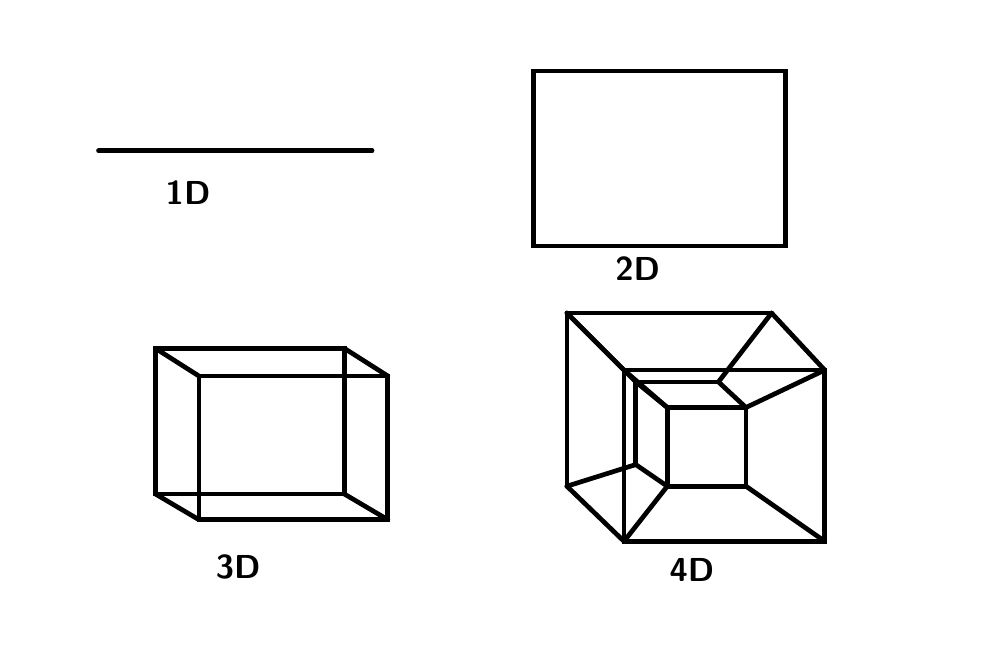
\begin{tikzpicture}[x=0.025cm, y=-0.025cm, line width=1.7pt, line cap=round,
                    lbl/.style={font=\fontsize{12}{12}\selectfont\sffamily\bfseries, inner sep=0pt}]

% full original canvas, including its (asymmetric) margins
\useasboundingbox (0,0) rectangle (482,305);

% ---- 1D: line ----
\draw (36,62.5) -- (175,62.5);
\node[lbl] at (81.5,84) {1D};

% ---- 2D: rectangle ----
\draw (257,22) rectangle (385,111);
\node[lbl] at (310,122.5) {2D};

% ---- 3D: cube (full wireframe, back face up-left) ----
\draw (65,163) rectangle (161,237);   % back face
\draw (87,177) rectangle (183,250);   % front face
\draw (65,163) -- (87,177)  (161,163) -- (183,177)
      (65,237) -- (87,250)  (161,237) -- (183,250);
\node[lbl] at (107,274) {3D};

% ---- 4D: tesseract (outer + inner cube, hidden lines removed) ----
% outer cube: front face A1..A4, back face B1(TL) B2(TR) B4(BL); B3 hidden
\coordinate (A1) at (303,174); \coordinate (A2) at (405,174);
\coordinate (A3) at (405,261); \coordinate (A4) at (303,261);
\coordinate (B1) at (274,145); \coordinate (B2) at (378,145);
\coordinate (B4) at (274,233);
% inner cube: front face a1..a4, back face b1(TL) b2(TR) b4(BL); b3 hidden
\coordinate (a1) at (325,193); \coordinate (a2) at (365,193);
\coordinate (a3) at (365,233); \coordinate (a4) at (325,233);
\coordinate (b1) at (309,180); \coordinate (b2) at (351,180);
\coordinate (b4) at (309,222);

\draw (A1) rectangle (A3);            % outer front face
\draw (B2) -- (B1) -- (B4);           % outer back face: top + left edges only
\draw (B1) -- (A1) (B2) -- (A2) (B4) -- (A4);   % outer corner edges
\draw (a1) rectangle (a3);            % inner front face
\draw (b2) -- (b1) -- (b4);           % inner back face: top + left edges only
\draw (b1) -- (a1) (b2) -- (a2) (b4) -- (a4);   % inner corner edges
% tesseract connectors, outer vertex -> inner vertex
\draw (B1) -- (b1) (B2) -- (b2) (B4) -- (b4)
      (A1) -- (a1) (A2) -- (a2) (A3) -- (a3) (A4) -- (a4);
\node[lbl] at (337.5,275.5) {4D};

\end{tikzpicture}
\end{document}
"
%   magick -density 600 1D-4D-rgb.pdf -background white -flatten ../../images/1D-4D.png
%   rm -f 1D-4D-rgb.pdf *.aux *.log
%
% The drawing is pure black, so the CMYK variant prints as 100% K ink.
\ifdefined\cmykcolors
  \PassOptionsToPackage{cmyk}{xcolor}
\else
  \PassOptionsToPackage{rgb}{xcolor}
\fi
\documentclass[border=0pt]{standalone}
\usepackage{fontspec}
\setsansfont{Arial}  % labels match the original raster's Arial; needs xelatex
\usepackage{tikz}

\begin{document}
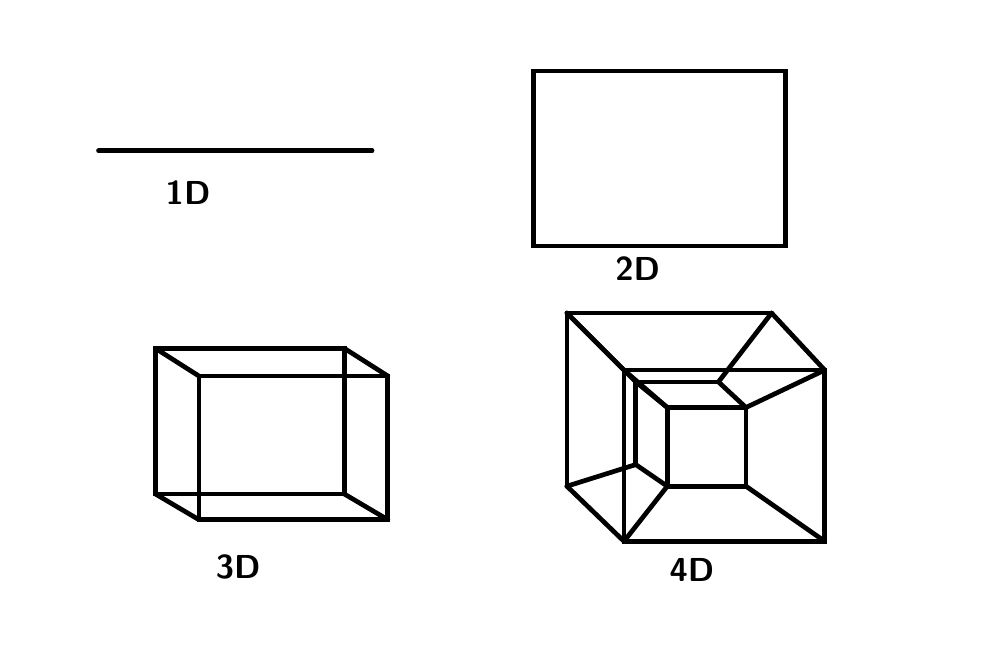
\begin{tikzpicture}[x=0.025cm, y=-0.025cm, line width=1.7pt, line cap=round,
                    lbl/.style={font=\fontsize{12}{12}\selectfont\sffamily\bfseries, inner sep=0pt}]

% full original canvas, including its (asymmetric) margins
\useasboundingbox (0,0) rectangle (482,305);

% ---- 1D: line ----
\draw (36,62.5) -- (175,62.5);
\node[lbl] at (81.5,84) {1D};

% ---- 2D: rectangle ----
\draw (257,22) rectangle (385,111);
\node[lbl] at (310,122.5) {2D};

% ---- 3D: cube (full wireframe, back face up-left) ----
\draw (65,163) rectangle (161,237);   % back face
\draw (87,177) rectangle (183,250);   % front face
\draw (65,163) -- (87,177)  (161,163) -- (183,177)
      (65,237) -- (87,250)  (161,237) -- (183,250);
\node[lbl] at (107,274) {3D};

% ---- 4D: tesseract (outer + inner cube, hidden lines removed) ----
% outer cube: front face A1..A4, back face B1(TL) B2(TR) B4(BL); B3 hidden
\coordinate (A1) at (303,174); \coordinate (A2) at (405,174);
\coordinate (A3) at (405,261); \coordinate (A4) at (303,261);
\coordinate (B1) at (274,145); \coordinate (B2) at (378,145);
\coordinate (B4) at (274,233);
% inner cube: front face a1..a4, back face b1(TL) b2(TR) b4(BL); b3 hidden
\coordinate (a1) at (325,193); \coordinate (a2) at (365,193);
\coordinate (a3) at (365,233); \coordinate (a4) at (325,233);
\coordinate (b1) at (309,180); \coordinate (b2) at (351,180);
\coordinate (b4) at (309,222);

\draw (A1) rectangle (A3);            % outer front face
\draw (B2) -- (B1) -- (B4);           % outer back face: top + left edges only
\draw (B1) -- (A1) (B2) -- (A2) (B4) -- (A4);   % outer corner edges
\draw (a1) rectangle (a3);            % inner front face
\draw (b2) -- (b1) -- (b4);           % inner back face: top + left edges only
\draw (b1) -- (a1) (b2) -- (a2) (b4) -- (a4);   % inner corner edges
% tesseract connectors, outer vertex -> inner vertex
\draw (B1) -- (b1) (B2) -- (b2) (B4) -- (b4)
      (A1) -- (a1) (A2) -- (a2) (A3) -- (a3) (A4) -- (a4);
\node[lbl] at (337.5,275.5) {4D};

\end{tikzpicture}
\end{document}
"
%   magick -density 600 1D-4D-rgb.pdf -background white -flatten ../../images/1D-4D.png
%   rm -f 1D-4D-rgb.pdf *.aux *.log
%
% The drawing is pure black, so the CMYK variant prints as 100% K ink.
\ifdefined\cmykcolors
  \PassOptionsToPackage{cmyk}{xcolor}
\else
  \PassOptionsToPackage{rgb}{xcolor}
\fi
\documentclass[border=0pt]{standalone}
\usepackage{fontspec}
\setsansfont{Arial}  % labels match the original raster's Arial; needs xelatex
\usepackage{tikz}

\begin{document}
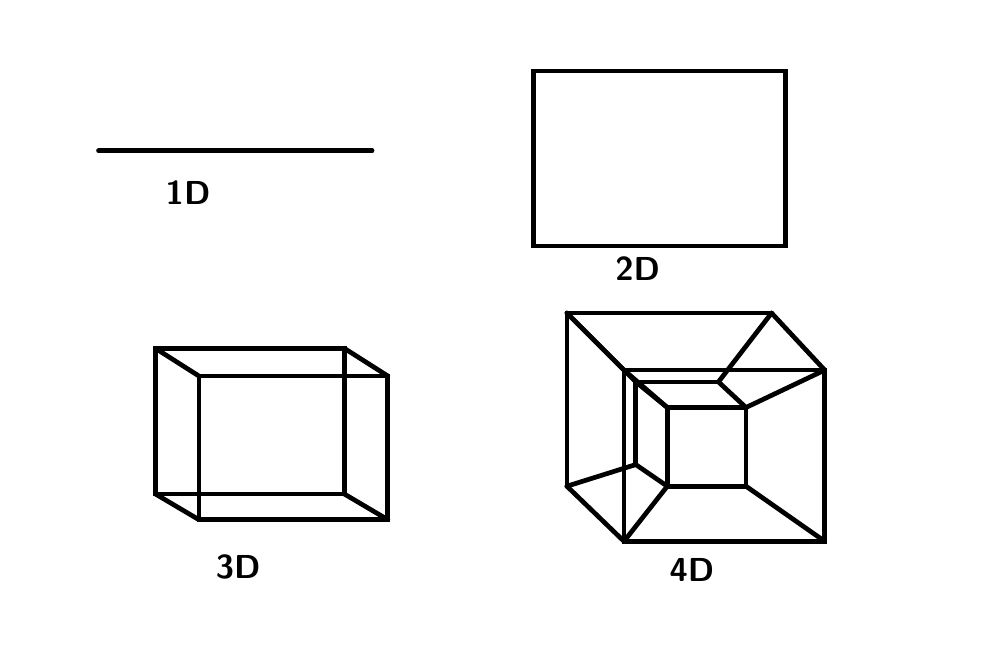
\begin{tikzpicture}[x=0.025cm, y=-0.025cm, line width=1.7pt, line cap=round,
                    lbl/.style={font=\fontsize{12}{12}\selectfont\sffamily\bfseries, inner sep=0pt}]

% full original canvas, including its (asymmetric) margins
\useasboundingbox (0,0) rectangle (482,305);

% ---- 1D: line ----
\draw (36,62.5) -- (175,62.5);
\node[lbl] at (81.5,84) {1D};

% ---- 2D: rectangle ----
\draw (257,22) rectangle (385,111);
\node[lbl] at (310,122.5) {2D};

% ---- 3D: cube (full wireframe, back face up-left) ----
\draw (65,163) rectangle (161,237);   % back face
\draw (87,177) rectangle (183,250);   % front face
\draw (65,163) -- (87,177)  (161,163) -- (183,177)
      (65,237) -- (87,250)  (161,237) -- (183,250);
\node[lbl] at (107,274) {3D};

% ---- 4D: tesseract (outer + inner cube, hidden lines removed) ----
% outer cube: front face A1..A4, back face B1(TL) B2(TR) B4(BL); B3 hidden
\coordinate (A1) at (303,174); \coordinate (A2) at (405,174);
\coordinate (A3) at (405,261); \coordinate (A4) at (303,261);
\coordinate (B1) at (274,145); \coordinate (B2) at (378,145);
\coordinate (B4) at (274,233);
% inner cube: front face a1..a4, back face b1(TL) b2(TR) b4(BL); b3 hidden
\coordinate (a1) at (325,193); \coordinate (a2) at (365,193);
\coordinate (a3) at (365,233); \coordinate (a4) at (325,233);
\coordinate (b1) at (309,180); \coordinate (b2) at (351,180);
\coordinate (b4) at (309,222);

\draw (A1) rectangle (A3);            % outer front face
\draw (B2) -- (B1) -- (B4);           % outer back face: top + left edges only
\draw (B1) -- (A1) (B2) -- (A2) (B4) -- (A4);   % outer corner edges
\draw (a1) rectangle (a3);            % inner front face
\draw (b2) -- (b1) -- (b4);           % inner back face: top + left edges only
\draw (b1) -- (a1) (b2) -- (a2) (b4) -- (a4);   % inner corner edges
% tesseract connectors, outer vertex -> inner vertex
\draw (B1) -- (b1) (B2) -- (b2) (B4) -- (b4)
      (A1) -- (a1) (A2) -- (a2) (A3) -- (a3) (A4) -- (a4);
\node[lbl] at (337.5,275.5) {4D};

\end{tikzpicture}
\end{document}
